

\section{Naming and The Filesystem Metaphore}
\label{chap:naming}

% From our experience with building applications, there are a clear set of requirements that are necessary.  
Most applications
construct the notion of context using the naming convention ascribed to a sensor stream.  The name conflates the notion of system,
space, and type information.  At the very least, these three should be supported, however, often other categorical needs must be
met to perform various kinds of aggregate statistical, analytics, and control.  In addition, we need to support the management of
processing jobs that process stream data and provide integrated management facilities for them.

Building applications are essentially monitoring and control applications built on the streams generated by sensors embedded through
the building or distillates of them.  As the number of applications and streams increased, it becomes desireable to manage them 
in a centralized fashion.  Moreover, the centralized apporach allows all applications to make use of a uniform naming convention and
can allow applications to be interoperable.  Systems that wish to support such applications require the following properties:

\begin{enumerate}
\item Logically accessible physical resources.
\item Representation of data producing and data consuming elements.
\item Representation of inter-relationships between elements.
\item Provide uniform naming and access.
\end{enumerate}

 
% We also discuss the incorporation of a pipe-like mechanism for 
% processing streams and their output.

\section{File Abstraction}

Our naming scheme is hierarchically structured, like traditional filesystem naming, with support
for symbolic links, allowing arbitrary links between sub-trees.  We argue that this naming scheme
is crucial, as it exposes the inter-relationships which inform aggregation semantics intended
by the user.  We introduce a naming scheme for physical objects and their inter-relationship.


% \vspace{0.08in}


Similar requirements to those aforementioned have been addressed in the design and implementation of filesystems.  Filesystems provide
logical access to physical resources through files, with different files and associated semantics, exposed to applications through a shell
or programmtically.  Filesystems representat collections of bits, encapsulated by a file, and grouped with folders.  Symbolic links support
the notion of multi-naming.  A single file or folder could have multiple names that lead to the same underlying object.  Filesystems even
support the notion of streaming data through character and block device files.  Moreover, pipe files allow programs to communite with each
other through a piece of shared memory, where the source application writes to the pipe and the sink application consumes from the pipe.

We assert that these constructs should be directly adopted for supporting applications in the buildings.  Our approach adopts the unix
file philosophy where everthing is represented as a file.  Each object created in StreamFS is assigned two names, by default, one which 
uniquely identifies the object and \emph{not} human-readable and the second which is changeable and human-readable.  Consider
the example shown in Figure~\cite{fig:everythingfile}.


\begin{figure}[t!] %htbp
\centering
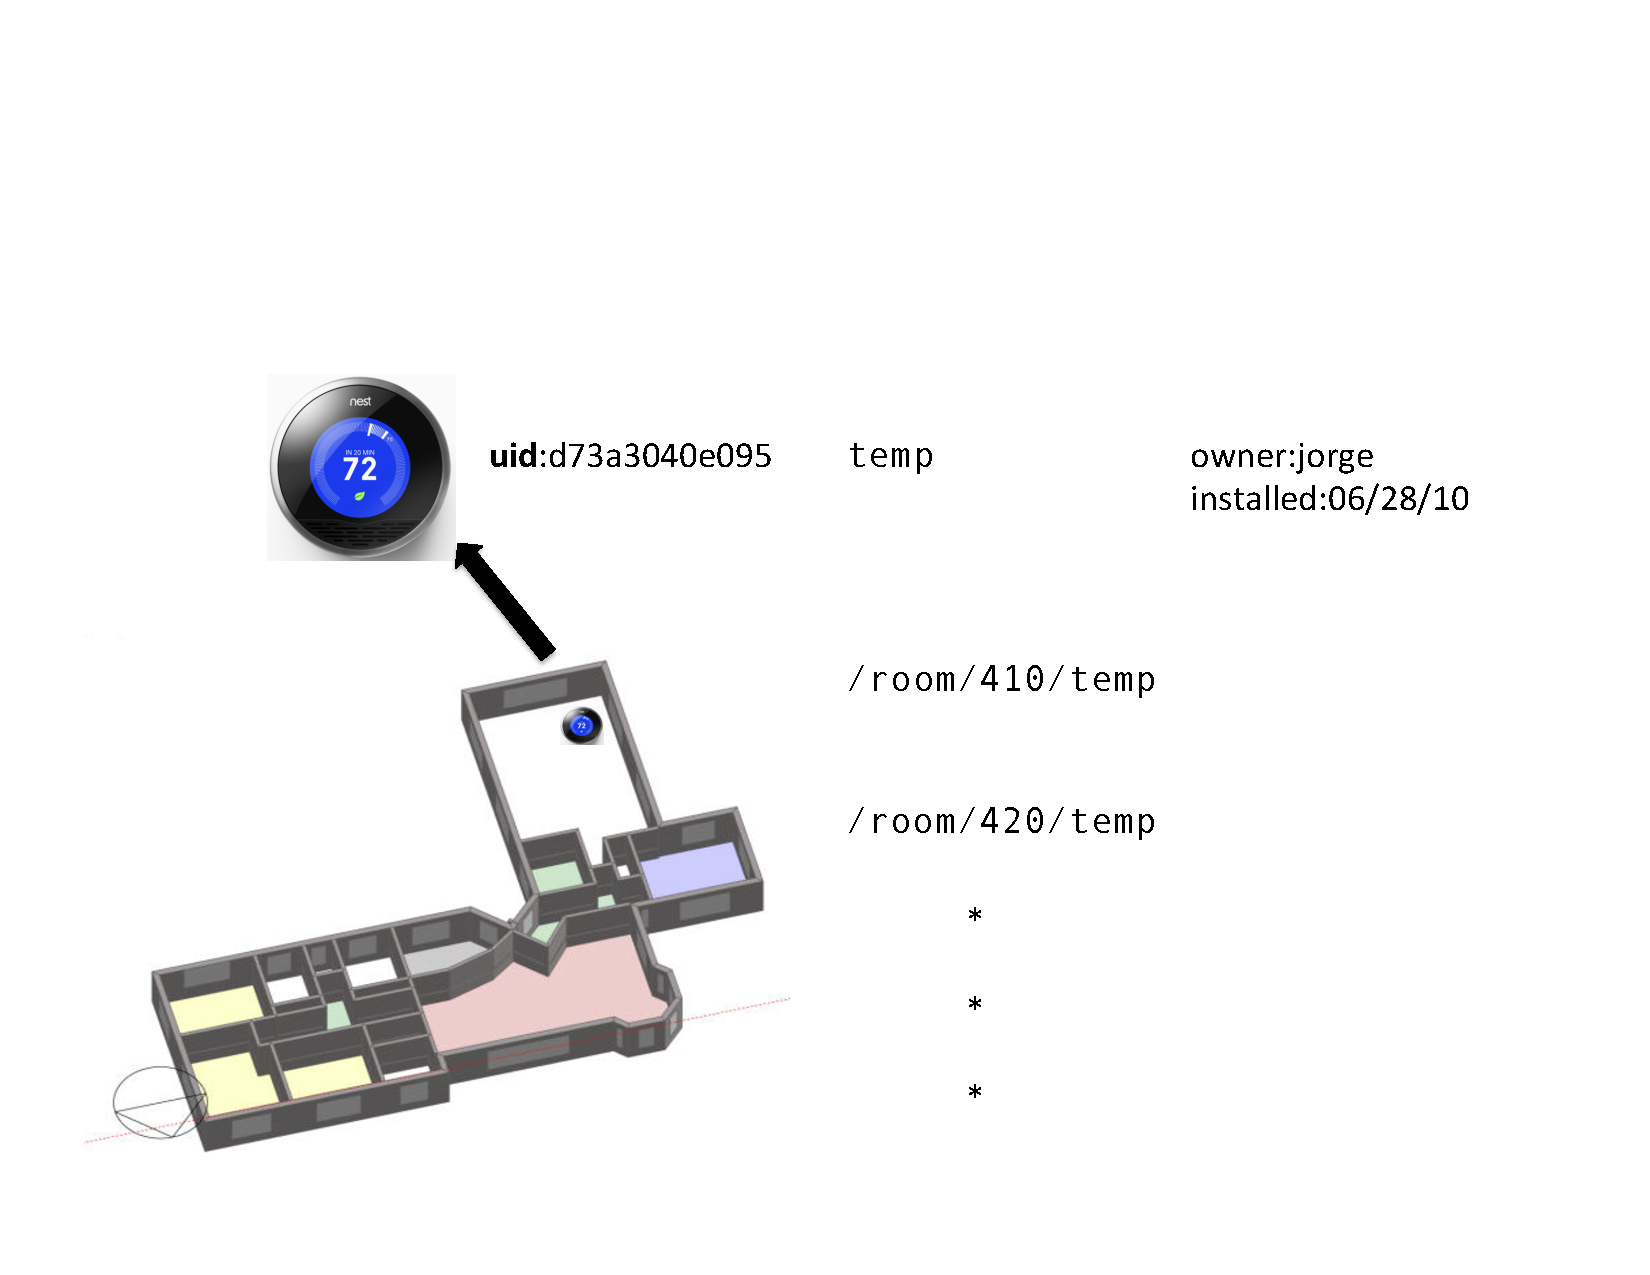
\includegraphics[width=0.65\columnwidth]{figs/everythingfile}
\caption{Everything is a file.  Temperature sensor represented as a file in a folder that contains folders for each room.
Note, the file that represents a temperature sensor producing a stream is given a unique identifer.  The user may also
decorate the file with extra metadata for searching purposes.}
\label{fig:everythingfile}
\end{figure}

In this example, the user is creating a temperature stream file in every room of the building.  The name of the file, given by the user,
is \emph{temp}.  Upon creation, the file is uniquely identified by the system using a unique identifier, as shown.  Like in a unix filesystem, the
file is created within a folder.  Ideally, the name of the folder would encode the placement of the sensor.  In the figure, the 
user is create a temperature stream file in room 410 and room 420.  Note the full filepath for the stream file is /room/410/temp.
During creation, the user may also decorate the file with extra metadata, also shown in the figure.  In this example, they have annotated
the file with information about the owner and when the sensor was installed.   This metadata is used for quickly locating the file
or grouping files that contain similar tags, quickly.

\subsection{File types and operations}
As we map the filesystem abstraction into this problem space, we need to consider the various kinds of files our system will contain,
their semantics, and how our system will expose and manage them.  There are essentially 4 types of files and 6 sub-types.  We summarize
these in Table~\ref{tab:filetypes}.  There are also different kinds of operations that the each file type supports.  Operational semantics
are file dependent.  For example, when you \emph{read} a folder, you obtain the metadata associated with the folder and the name
of its children.  When you \emph{read} a stream, you its metadata and the last timestamp-value it produced.  \emph{Writ}ing to a stream
is a bit different.  You can write to a stream to update its metadata tags and the stream source can write a value to it.  The stream
source is identified with a \emph{publish identifier} (pubid).  The stream source includes the pubid in the write operation for 
the specified stream file.  Without the pubid, the source cannot write to the file.  Any other writer should not be allowed to write to 
a stream file either.  

\begin{table}[h]
\begin{center}
\begin{tabular}{| r | l | l |}
	\hline
	\textbf{type} & \textbf{description} & \textbf{valid operations} \\ \hline
	default/folder & Container file.  Used to group other  & read, write, delete  \\
				   & kinds of files within it.  &  \\ \hline

	stream & Represents a data stream. & read, write, delete, subscribe, \\
			&							&query \\ \hline

	controller & Represents a controller. & read, write, subscribe \\ \hline

	special & There are several kinds of special files for  & read, delete \\
		    & management of jobs and pipes. &  \\ 
	\hline
\end{tabular}
\caption{Summary of the 4 main file types and their valid operations in StreamFS.}
\label{tab:filetypes}
\end{center}
\end{table}

Similar to a traditional filesystem, StreamFS includes \emph{special files}.  There are 6 special files and 5 of them 
are for management purposes.  The only one that is not is the \emph{symbolic link} file, which is essentially used to support
multi-naming and inherents the operational semantics of the file it points to.  The delete operation on a symlink, however,
only deletes the symlink.  A description of these files and the operations they support is given in Table~\ref{tab:filesubtypes}.
A detailed description and examples with be presented in later sections.


\begin{table}[h]
\begin{center}
\begin{tabular}{| r | l | l |}
	\hline
	\textbf{operation} & \textbf{file type} & \textbf{semantics} \\ \hline
	read & folder, stream, ipd, ipi, epd, epi, sub & read the metadata and tags for \\
		 &										   & the associated file. \\ \hline
	write &  stream & Write to stream file, only the \\ 
		  & 		& appropiate stream source is permitted.\\ \hline
	delete & folder, stream, ipd, ipi, epd, epi, sub & Folder must be empty.  \\
		   & 										 & The others can be directly deleted. \\ \hline
	query &  stream, all & streams support time-range queries.  \\
		  &			     & All support metadata-tag queries.\\ \hline
	subscribe & stream & Forwards data from a stream to the\\
			  &		   & specified destination.\\
	\hline
\end{tabular}
\caption{File opertaitons, the file types that support them, and their general semantics.}
\label{tab:semantics}
\end{center}
\end{table}

\subsection{Default, Stream, and Controller Files}
% \subsection{Default/Folder Files}
A default or folder file serve primarily as a container for other kinds of files.  It is used to group together different kinds of file and
to represent a common attribute of the file within it.  For example, a default file is usually used to construct the spatial hierarchy.
Each file at the top level represents a floor, its children are also a set of default file, representing each of the rooms on that floor.
A default file cannot be deleted unless it is empty.

File that represent streams are called stream files.  They are tightly associated with the associated stream data in the timeseries data-store.
A user created a stream file and that associated stream ``writes'' to it in order to have its data saved.  StreamFS also forwards the
data to the \emph{subscription manager} in case any subscription sink has subscribed to this feed.  When a stream file is create an id is 
returned to the user.  This id must be used by the stream that wishes to push its data to StreamFS through this file.  If this id is incorrect
or not include, the write operation is rejected.

Because controllers accpet many kinds of input, we designed the the file that presents a controller similar to the external processing stub discussed
in section~\ref{sec:externalprocs}.  Writes to a controller file and forwarded directly to the control stub running at the controller itself or a proxy
machine that communicates with the controller.  Any reply is set as metadata in the controller file.  Controller files also an associated output stream.
If a controller process wishes to inform the process of internal state at the controller, it does so through the controller file output --
a stream file itself.  Table~\ref{tab:filetypes} lists the files in streamfs and the operations they support.  The operational semantics
are listed in Table~\ref{tab:semantics}.

% \subsection{Stream Files}

% \subsection{Controller Files}

\subsection{Special Files}
There are 6 types of special files.  In chapter~\ref{chap:ProcMngtSchedMain} we eluded to the various kinds of file that are created
when a user creates an internal or external file.  An internal process definition (ipd) file is created when the user
submits a script to StreamFS.  When a (set of) stream(s) is piped through the defintion file, an internal process instance (ipi) file
is created that represents the output of the process.  A subscription instance (sub) file is also created.  The sub file contains
information about which streams are feed the file, a reference to the ipi file, and statistics about the file.  If either
the sub file or the ipi file are deleted, the process ends.  The ipi file is also a stream file.  It can be used to pipe that
output of the process to another processes or to an external \texttt{URL}.

\begin{table}[h]
\begin{center}
\begin{tabular}{| l | l | l |}
	\hline
	\textbf{type} & \textbf{description} & \textbf{valid operations} \\ \hline
	
	internal process  & Javascript process definition.  & read, write, delete  \\ 
	defintion (ipd)   & 							    &	\\ \hline

	internal process  & Management file used for managing & read, delete \\
	instance (ipi)	  & active processing of this script. & \\ \hline

	external process  & Gives information about where an & read, write, delete \\
	definition (epd)  & external process lives. &\\ \hline

	external process  & An active processing stream to an  & read, write, delete \\
	instance (epi)	  & external process. &\\ \hline

	subscription instance & An instance of a subscription.  Contains & read, delete \\
				(sub) 	  & information about the subscription, &\\
								& such as source/sink and related statistics &\\ \hline
								
	symbolic link (symlink) & Similar to a symbolic link in Unix. & \\
	\hline
\end{tabular}
\caption{Summary of the 6 special-file sub-types and their valid operations in StreamFS.}
\label{tab:filesubtypes}
\end{center}
\end{table}

The same set of files are created when an external processes is defined and started.  When the client stub is started on the client
machines it creates an external procrocess definition file for each process that was listed in the configuration file for the stub on 
the client machine.  Similarly, when streams are piped to the defintion files, the client starts the processes on the client
and create their associated external process instance (epi) files.  Those files are also a sub-type of the stream file and can
be used to pipe the output to another process (internal or external) or an external \texttt{URL}.
Any subscription or pipe that is instantiated creates an associated sub file in the \texttt{/sub} directory.  These always contain information
about the subscription and kill the fowarding process when deleted.

Finally, we used symbolic link (symlinks) the same way they are used in a traditional filesystem.  They are also used to generalize
the inter-relationship structure in the ERG.  They are a crucial file in the support of multi-naming.

% \subsection{Special Files}

% \subsubsection{Internal Process Definition}
% \subsubsection{Internal Process Instance}
% \subsubsection{External Process Definition}
% \subsubsection{External Process Instance}
% \subsubsection{Subscription Instance}










\section{Supporting Multiple Names}

One of the goals of the naming scheme in StreamFS is to support multiple names for sensor and actuators.  The inclusion of symlinks 
provides this ability.  A file can be named and linked to from multiple hierarchies.  This allows applications to refer
to the same physical entity with a unique object id through multiple names.  It is also used by our pub-sub system when
the names are resolved and play a crucial role in \emph{dynamic aggregation}.

For example, a temperature sensor may have at least two names that are expose to the end user.  It may have a name that refers to 
it through the context of its spatial placement, such as \texttt{/soda/4F/410R/temp} and it may have a name that refers to it 
through the context of its association with a component in the HVAC system, such as \texttt{/soda/hvac/ahu1/vent1/temp}.  Either
of those are names that should access the same item and that item's associated data.  The underlying stream may actually write
the data to a stream file named \texttt{/strms/temp} and the other two names are just symlinks to this one.  

The pub-sub system uses these names when decided which data streams match a subscription topic.  For example, in a typical pub-sub system,
if a job wanted to subscribe to the temp stream, it would have to know the name \emph{a priori}, or simply pick a single name.
However, we support the notion of multi-topic stream tags.  So, if a subscriber request all the streams with the topic 
\texttt{/soda/4F/410R/*} and a data point is written to \texttt{/strm/temp}, the subscription manager would list all the aliases
for that name, which include \texttt{/soda/4F/410R/temp} and see that it matches the topic request for that subscription.

Notice how naming explicitly affects how we group sensors according to some hiearchical organization.  Some of those groupings
are physical associations with one another that are important to stay accurate.  Let's re-examine the example presented in
Section~\ref{sec:cntxtacc}.  We present the figure from that section again in Figure~\ref{fig:mpc_example2}.

% walk through the example and show how multinaming helps address this and 
% why it's important to get right -- that should lead us right into the next section with no problem.

\begin{figure}[h!] %htbp
\centering
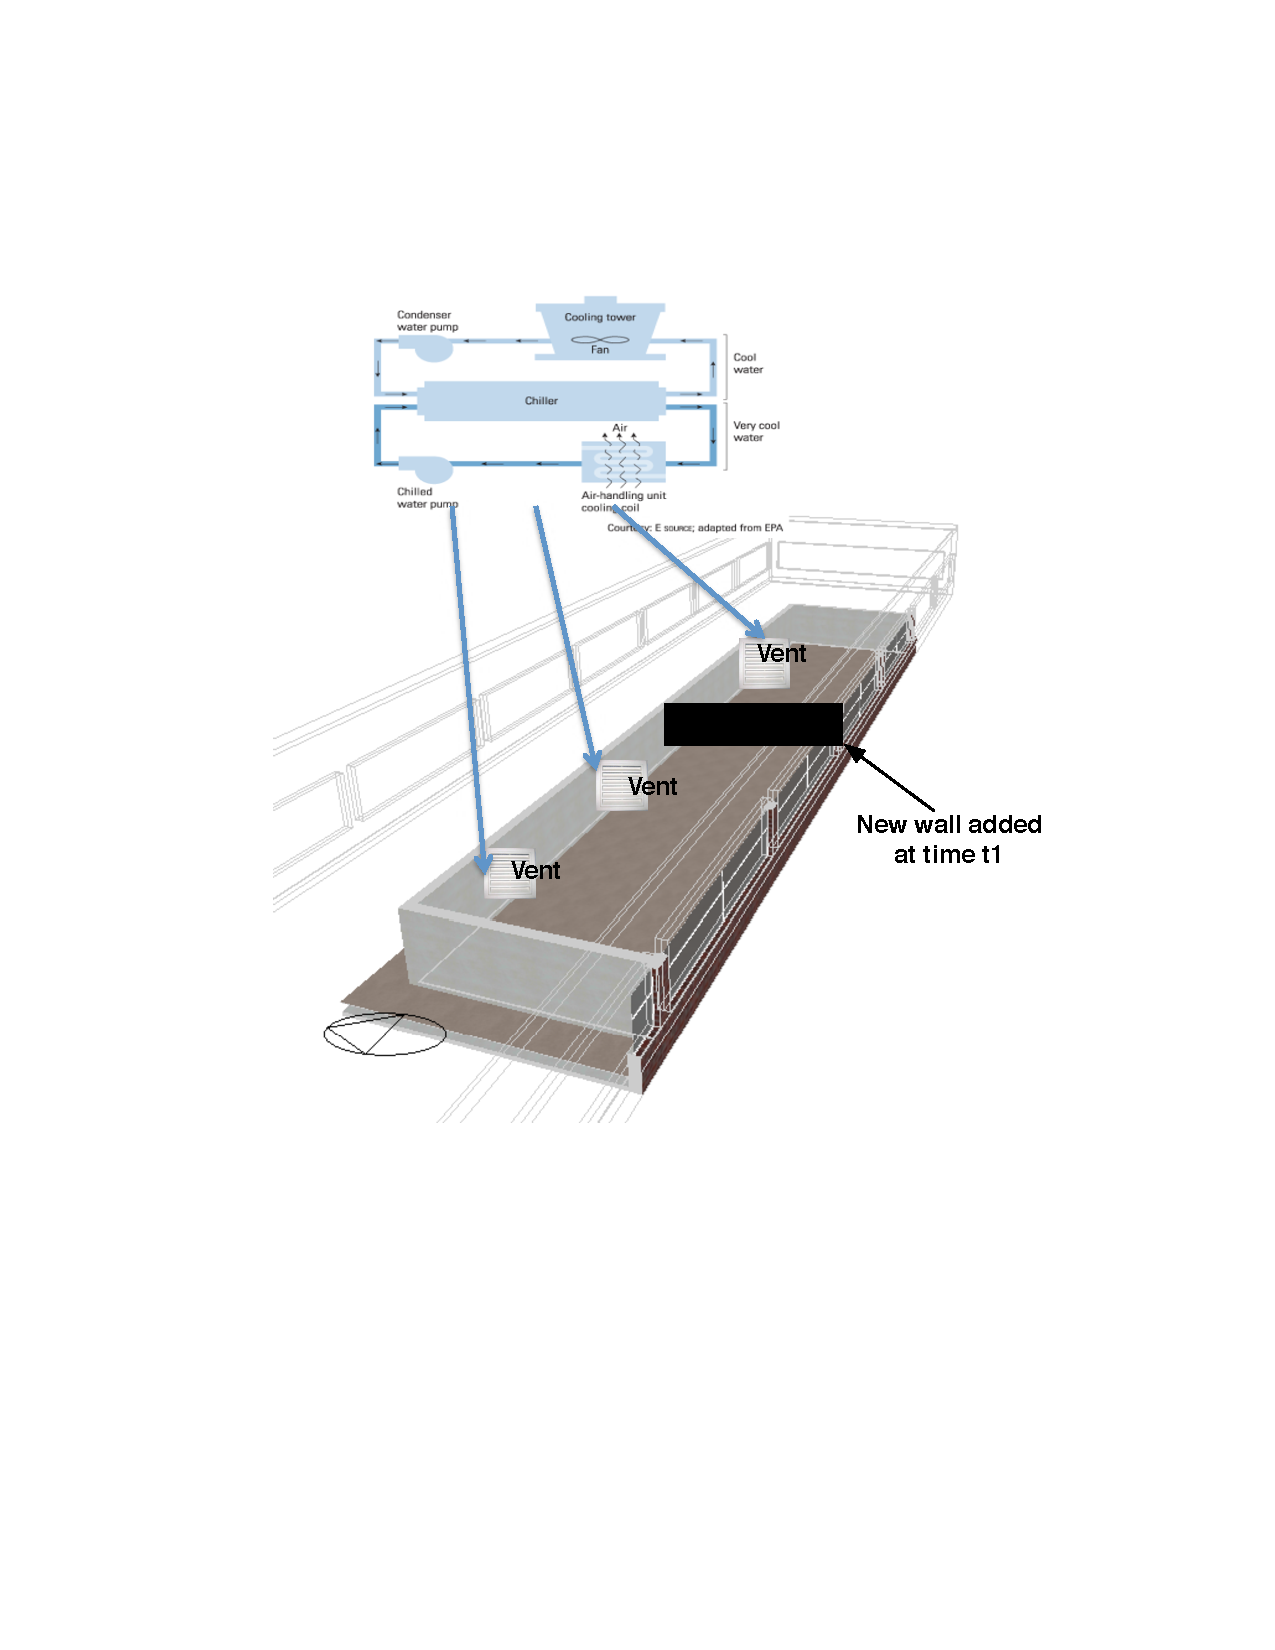
\includegraphics[width=0.5\columnwidth]{figs/mpc_example}
\caption{MPC example where metadata must be verified to maintain correct behavior.}
\label{fig:mpc_example2}
\end{figure}

Recall that the equation that drives the control process depends on knowing the mapping between vents and rooms.  Therefore,
if the room changes and a vent is added or removed, the control algorithm must be updated to account for the change.  The naming
structure would contain a reference to the vent in some group, linked to a sensor that belongs to a certain room, however,
if a wall is put up, we should be able to automatically detect that this has occurred to update the control process.
In summary, the naming scheme is used to express different kinds of organizational patterns for the sensors and their data.
As the building goes through some changes and evolves an automatic scheme or family of schemes are necessary to alert
the user or process of the chance.  In the next
section we discuss the mathematical tools we used to verify that the groups specified by the naming convention are correct.

% \section{Verification through Sensor Data}
Verification is a broad topic in buildings that refers to verifying several things about building sensor metadata or through
the sensor data.  Both cases are related to physical states are relationships that are assumed by the user and are either
true and empirically observable or not.  If not, the end user or process should be informed and that inconsistencies should
be immediately addressed.  This is even more of an issues as building begin to reply more and more on software.

In this section we introduce some of the tools that we use for verification as discuss the 4 types of verification
that exists in buildings.  We also present an overview approach for 3 of them.

\subsection{Correlation}
Throughout this work, we make extensive use of the correlation coefficient function defined as: 

\begin{displaymath}
r(X,Y) = r_{X, Y} = \frac{\sum_{i=1}^{n} (X_{i} - \overline{X})(Y_{i} - \overline{Y})}
{\sqrt{\sum_{i=1}^{n} (X_{i} - \overline{X})^2}\sqrt{\sum_{i=1}^{n} (Y_{i} - \overline{Y})^2}}
\end{displaymath}

where $X$, $Y$ are separate sets of values, $n$ is the total number of sample points in 
each set, and $\overline{X}$ is the mean value of $X$ (same for $\overline{Y}$ and Y).  % over the entire sampling period.
For each pair of sensors, we compute the corrcoeff to ascertain the relationship between them.


\subsection{Empirical Mode Decomposition} \label{emd}
Another important tool that we used is empirical mode decomposition.  We use it partition the empiriical data is its constituent
sub-signals and examine what those sub-signals tell us about its behavior.  We also use it to examine how signal behavve between
one another at certain bands of importance that contain important physical information.

Empirical Mode Decomposition (EMD) \cite{huang:emd1998} is a technique that decomposes a signal and reveals intrinsic patterns, 
trends, and noise.
This technique has been widely applied to a variety of datasets, including climate variables~\cite{lee:climateEMD2011}, medical data~\cite{blanco:bioMed2008}, speech signals~\cite{huang:signalProc2006,hasan:ieeeletter2009}, and image processing~\cite{nunes:vision2005}.
% for example, it helped to uncover the global surface temperature trends\cite{}, solar activity patterns and predicts climate variables .
EMD's effectiveness relies on its empirical, adaptive and intuitive approach.
In fact, this technique is designed to efficiently decompose both non-stationary and non-linear signals without requiring any 
a priori basis functions or tuning.  

EMD decomposes a signal into a set of oscillatory components called intrinsic mode functions (IMFs). 
An IMF satisfies two conditions: (1) it contains the same number of extrema and zero crossings (or differ at most by one); (2) the two 
IMF envelopes defined by its local maxima and local minima are symmetric with respect to zero.  Consequently, 
 IMFs are functions that directly convey the amplitude and frequency modulations.

% EMD is an iterative sifting process that extracts IMFs step by step; each step seeks for the IMF with the highest frequency, then the computed IMF is removed from the data and the residual data are used as input for the next step.
EMD is an iterative algorithm that extracts IMFs step by step by using the so-called sifting process \cite{huang:emd1998}; each step seeks for the IMF with the highest frequency by sifting, then the computed IMF is removed from the data and the residual data are used as input for the 
next step.
The process stops when the residual data becomes a monotonic function from which no more IMF can be extracted.

We formally describe the EMD algorithm as follows: 
\begin{enumerate}
\item Sifting process: For a current signal $h_0=X$, let $m_0$ be the mean of its upper and lower envelopes as determined from a cubic-spline interpolation of local maxima and minima.
\item The estimated local mean $m_0$ is removed from the signal, giving a first component: $h_1 = h_0-m_0$
\item The sifting process is iterated, $h_1$ taking the place of $h_0$. Using its upper and lower envelopes, a new local mean $m_1$ is computed and $h_2 = h_1-m_1$.
\item The procedure is repeated $k$ times until $h_k=h_{k-1}-m_{k-1}$ is an IMF according to the two conditions above.
\item This first IMF is designated as $c_1 = h_k$, and contains the component with shortest periods. We extract it from the signal to produce a residual: $r_1 = X - c_1$.  Steps 1 to 4 are repeated on the residual signal $r_1$, providing IMFs $c_j$ and residuals $r_j  = r_{j-1}-c_j$, for $j$ from $1$ to $n$.
\item The process stops when residual $r_n$ contains no more than 3 extrema.
\end{enumerate}

The result of EMD is a set of IMFs $c_i$ and the final residue $r_n$, such as: \[X=\sum^{n}_{i=1}c_i+r_n\]
where the size of the resulting set of IMFs ($n$) depends on the original signal $X$ and $r_n$ represents the trend of 
the data (see \emph{IMFs} in Figure~\ref{fig:diagram1}).

For this work we implemented a variant of EMD called Complete Ensemble EMD~\cite{torres:icassp2012}.
This algorithm computes EMD several times with additional noise, it allows us to efficiently analyze signals that have 
flat sections (i.e. consuming no electricity in our case). % and permits us to solve the \emph{EMD mode mixing problem}.

\subsection{Reaggregation of Intrinsic Mode Functions} \label{methodo:corr}
By applying EMD to energy consumption signals we obtain a set of IMFs that precisely describe the devices consumption 
patterns at different frequency bands.  Therefore, we can focus our analysis on the smaller time scales, ignoring the dominant 
patterns that prevent us from effectively analyzing raw signals.

However, comparing the IMFs obtained from different signals is also not trivial,
 because EMD is empirically uncovering IMFs from the data there is no guarantee that the two IMFs $c_i^1$ and $c_i^2$ obtained from two distinct signals $S^1$ and $S^2$ represent data at the same frequency domain.
Directly comparing $c_i^1$ and $c_i^2$ is meaningless unless we confirm that they belong to the same frequency domain.

There are numerous techniques to retrieve IMF frequencies~\cite{huang:aada2009}.  
In this work we take advantage of the Generalized Zero Crossing (GZC)~\cite{huang:patent2006} because it is a simple and robust 
estimator of the instantaneous IMF frequency \cite{huang:aada2009}.
GZC is a direct estimation of IMF instantaneous frequency using critical points defined as the zero crossings and local extrema 
(round dots in Figure~\ref{fig:gzc}).
Formally, given a data point $p$, GZC measures the quarter ($T_4$), the two halves ($T_2^x$), and the four full periods ($T_1^y$), $p$   
belong to (see Figure~\ref{fig:gzc}) and the instantaneous period is computed as:
\[T=\frac{1}{7}\{4T_4+(2T_2^1+2T_2^2)+(T_1^1+T_1^2+T_1^3+T_1^4)\}\]

\begin{figure}
\begin{center}
 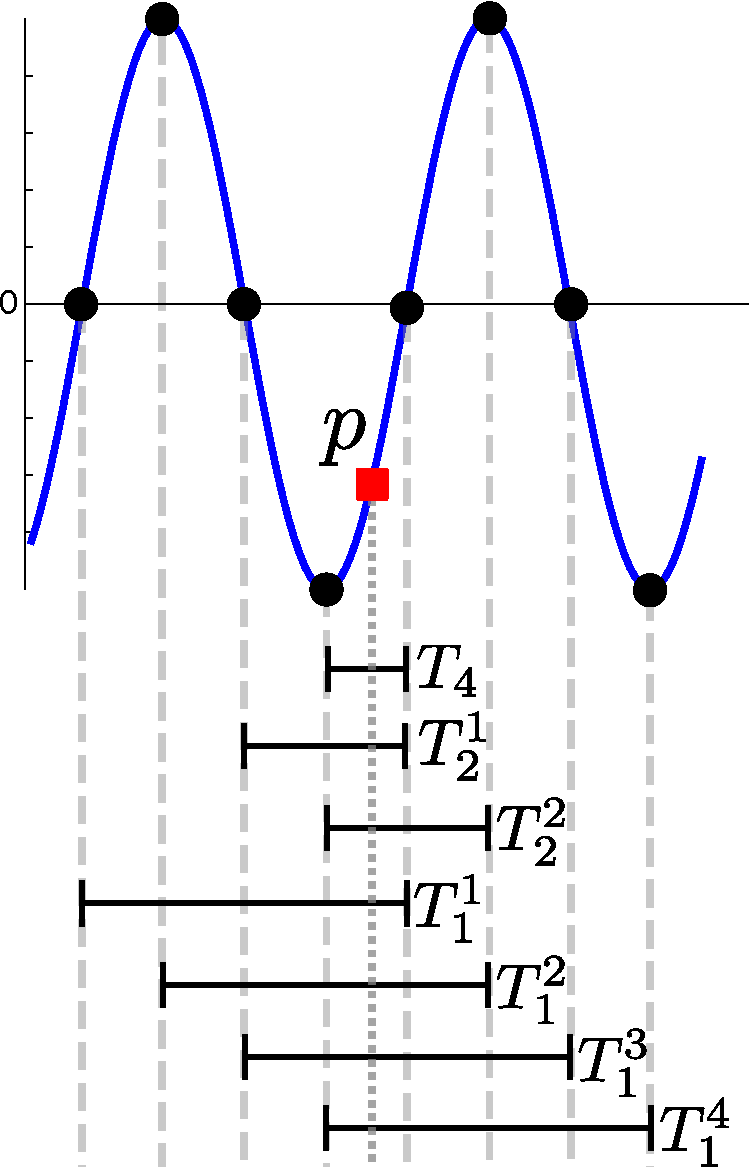
\includegraphics[width=.25\textwidth]{figs/gzc.pdf}
 \end{center}
 \caption{Generalized Zero Crossing: the local mean period at the point $p$ is computed from one quarter period $T_4$, two half periods $T_2^x$ and four full periods $T_1^y$ (where $x=1, 2$, and, $y=1,2,3,4$).}
 \label{fig:gzc}
\end{figure}

Since all points $p$ between two critical points have the same instantaneous period GZC is local down to a quarter period.
Hereafter, we refer to the time scale of an IMF as the average of the instantaneous periods along the whole IMF.
Because the time scale of each IMF depends on the original signal, we propose the following to efficiently compare IMFs from different signals.
We cluster IMFs with respect to their time scales and partially reconstruct each signal by aggregating its IMFs from the 
same cluster.  Then, we directly compare the partial signals of different devices.

EMD yields distinct components in different time scales and we compute the instantaneous frequencies \cite{IF} of IMFs using Generalized Zero-Crossing \cite{GZC}.  We break the time scales into four frequency bands:
\begin{itemize}
\item High Frequency: a time scale smaller than 30 minutes, mainly reflecting the operation characteristics of devices and noise in system. 
\item Medium Frequency: a time scale between 30 minutes and 6 hours, which is within the time span of daily activities inside a building.
\item Low Frequency: a time scale between 6 hours and 7 days. %This category usually captures patterns repeated in a longer cycle, say, days. 
\item Residue: everything has a time scale longer than 7 days and shows long-term patterns, such as seasonal changes.
\end{itemize}

Later in this thesis we will explain how we use the medium-frequency band for both spatial verification and functional verification.  We discuss
the 4 types of verification in the next section.






% \section{Types of Verification}
There are 3 kinds of verification that we discuss in this section.

\begin{enumerate}
\item \emph{Functional}: verifying whether the behavior of the components in changing.
\item \emph{Spatial}: 	verifying the spatial relationship between components.
\item \emph{Categorical}: verifying the unit of measure and phenomenon being observed.
% \item Value
\end{enumerate}

Before we discuss the details and approach for each, let us first examine the mathematical tools that we
use in our solutions.  Then we discuss each type of verification in more detail.  We give a detailed description 
of the methodology for each and present the results of our analysis.

\subsection{Correlation}
Throughout this work, we make extensive use of the correlation coefficient function defined as: 

\begin{displaymath}
r(X,Y) = r_{X, Y} = \frac{\sum_{i=1}^{n} (X_{i} - \overline{X})(Y_{i} - \overline{Y})}
{\sqrt{\sum_{i=1}^{n} (X_{i} - \overline{X})^2}\sqrt{\sum_{i=1}^{n} (Y_{i} - \overline{Y})^2}}
\end{displaymath}

where $X$, $Y$ are separate sets of values, $n$ is the total number of sample points in 
each set, and $\overline{X}$ is the mean value of $X$ (same for $\overline{Y}$ and Y).  % over the entire sampling period.
For each pair of sensors, we compute the corrcoeff to ascertain the relationship between them.


\subsection{Empirical Mode Decomposition} \label{emd}
Another important tool that we used is empirical mode decomposition.  We use it partition the empirical data is its constituent
sub-signals and examine what those sub-signals tell us about its behavior.  We also use it to examine how signals behave between
one another at certain bands of importance that contain important physical information.

Empirical Mode Decomposition (EMD) \cite{huang:emd1998} is a technique that decomposes a signal and reveals intrinsic patterns, 
trends, and noise.
This technique has been widely applied to a variety of datasets, including climate variables\cite{climate}, medical 
data\cite{blanco:bioMed2008}, speech signals\cite{huang:signalProc2006,hasan:ieeeletter2009}, and image processing~\cite{nunes:vision2005}.
% for example, it helped to uncover the global surface temperature trends\cite{}, solar activity patterns and predicts climate variables .
EMD's effectiveness relies on its empirical, adaptive and intuitive approach.
In fact, this technique is designed to efficiently decompose both non-stationary and non-linear signals without requiring any 
a priori basis functions or tuning.  

EMD decomposes a signal into a set of oscillatory components called intrinsic mode functions (IMFs). 
An IMF satisfies two conditions: (1) it contains the same number of extrema and zero crossings (or differ at most by one); (2) the two 
IMF envelopes defined by its local maxima and local minima are symmetric with respect to zero.  Consequently, 
 IMFs are functions that directly convey the amplitude and frequency modulations.

% EMD is an iterative sifting process that extracts IMFs step by step; each step seeks for the IMF with the highest frequency, then the computed IMF is removed from the data and the residual data are used as input for the next step.
EMD is an iterative algorithm that extracts IMFs step by step by using the so-called sifting 
process \cite{huang:emd1998}; each step seeks for the IMF with the highest frequency by sifting, then 
the computed IMF is removed from the data and the residual data are used as input for the 
next step.
The process stops when the residual data becomes a monotonic function from which no more IMF can be extracted.

We formally describe the EMD algorithm as follows: 
\begin{enumerate}
\item Sifting process: For a current signal $h_0=X$, let $m_0$ be the mean of its upper and lower envelopes as determined from a cubic-spline interpolation of local maxima and minima.
\item The estimated local mean $m_0$ is removed from the signal, giving a first component: $h_1 = h_0-m_0$
\item The sifting process is iterated, $h_1$ taking the place of $h_0$. Using its upper and lower envelopes, a new local mean $m_1$ is computed and $h_2 = h_1-m_1$.
\item The procedure is repeated $k$ times until $h_k=h_{k-1}-m_{k-1}$ is an IMF according to the two conditions above.
\item This first IMF is designated as $c_1 = h_k$, and contains the component with shortest periods. We extract it from the signal to produce a residual: $r_1 = X - c_1$.  Steps 1 to 4 are repeated on the residual signal $r_1$, providing IMFs $c_j$ and residuals $r_j  = r_{j-1}-c_j$, for $j$ from $1$ to $n$.
\item The process stops when residual $r_n$ contains no more than 3 extrema.
\end{enumerate}

The result of EMD is a set of IMFs $c_i$ and the final residue $r_n$, such as: \[X=\sum^{n}_{i=1}c_i+r_n\]
where the size of the resulting set of IMFs ($n$) depends on the original signal $X$ and $r_n$ represents the trend of 
the data (see \emph{IMFs} in Figure~\ref{fig:diagram1}).

For this work we implemented a variant of EMD called Complete Ensemble EMD~\cite{torres:icassp2012}.
This algorithm computes EMD several times with additional noise, it allows us to efficiently analyze signals that have 
flat sections (i.e. consuming no electricity in our case). % and permits us to solve the \emph{EMD mode mixing problem}.

\subsection{Reaggregation of Intrinsic Mode Functions} \label{methodo:corr}
By applying EMD to energy consumption signals we obtain a set of IMFs that precisely describe the devices consumption 
patterns at different frequency bands.  Therefore, we can focus our analysis on the smaller time scales, ignoring the dominant 
patterns that prevent us from effectively analyzing raw signals.

However, comparing the IMFs obtained from different signals is also not trivial,
 because EMD is empirically uncovering IMFs from the data there is no guarantee that the two IMFs $c_i^1$ and $c_i^2$ obtained from two distinct signals $S^1$ and $S^2$ represent data at the same frequency domain.
Directly comparing $c_i^1$ and $c_i^2$ is meaningless unless we confirm that they belong to the same frequency domain.

There are numerous techniques to retrieve IMF frequencies~\cite{IF}.  
In this work we take advantage of the Generalized Zero Crossing (GZC)~\cite{GZC} because it is a simple and robust 
estimator of the instantaneous IMF 
frequency\cite{IF}.
GZC is a direct estimation of IMF instantaneous frequency using critical points defined as the zero crossings and local extrema 
(round dots in Figure~\ref{fig:gzc}).
Formally, given a data point $p$, GZC measures the quarter ($T_4$), the two halves ($T_2^x$), and the four full periods ($T_1^y$), $p$   
belong to (see Figure~\ref{fig:gzc}) and the instantaneous period is computed as:
\[T=\frac{1}{7}\{4T_4+(2T_2^1+2T_2^2)+(T_1^1+T_1^2+T_1^3+T_1^4)\}\]

\begin{figure}
\begin{center}
 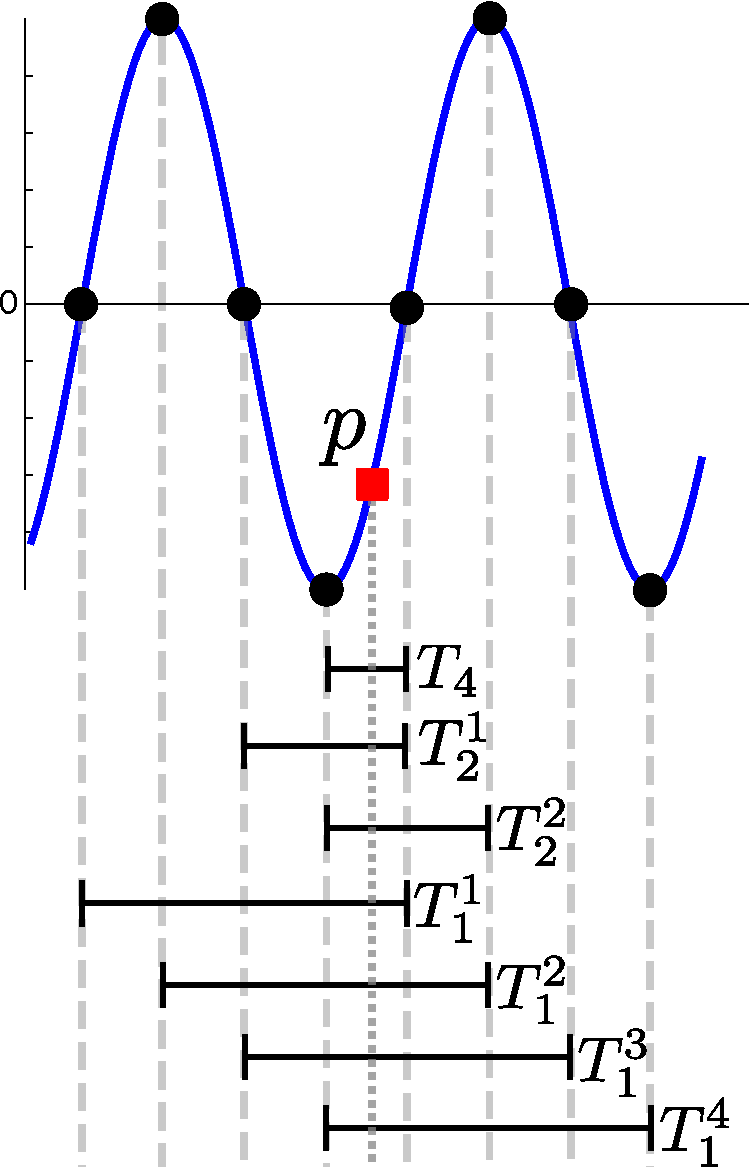
\includegraphics[width=.25\textwidth]{figs/gzc.pdf}
 \end{center}
 \caption{Generalized Zero Crossing: the local mean period at the point $p$ is computed from one quarter period $T_4$, two half periods $T_2^x$ and four full periods $T_1^y$ (where $x=1, 2$, and, $y=1,2,3,4$).}
 \label{fig:gzc}
\end{figure}

Since all points $p$ between two critical points have the same instantaneous period GZC is local down to a quarter period.
Hereafter, we refer to the time scale of an IMF as the average of the instantaneous periods along the whole IMF.
Because the time scale of each IMF depends on the original signal, we propose the following to efficiently compare IMFs from different signals.
We cluster IMFs with respect to their time scales and partially reconstruct each signal by aggregating its IMFs from the 
same cluster.  Then, we directly compare the partial signals of different devices.

EMD yields distinct components in different time scales and we compute the instantaneous frequencies \cite{IF} of IMFs using Generalized Zero-Crossing \cite{GZC}.  We break the time scales into four frequency bands:
\begin{itemize}
\item High Frequency: a time scale smaller than 30 minutes, mainly reflecting the operation characteristics of devices and noise in system. 
\item Medium Frequency: a time scale between 30 minutes and 6 hours, which is within the time span of daily activities inside a building.
\item Low Frequency: a time scale between 6 hours and 7 days. %This category usually captures patterns repeated in a longer cycle, say, days. 
\item Residue: everything has a time scale longer than 7 days and shows long-term patterns, such as seasonal changes.
\end{itemize}

Later in this thesis we will explain how we use the medium-frequency band for both spatial verification and functional verification.  We discuss
the 4 types of verification in the next section.







\subsection{Functional Verification}% With Strip, Bind, and Search}
% A typical large building contains thousands of sensors, monitoring the HVAC system, lighting, and other operational sub-systems.
With an increased push for operational efficiency, operators are relying more on historical data processing to uncover opportunities for energy-savings.
However, they are overwhelmed with the deluge of data and seek more efficient ways to identify potential problems.
In this thesis, we present an approach called the Strip, Bind and Search (SBS); a method for uncovering abnormal 
equipment behavior and in-concert usage patterns.
SBS uncovers relationships between devices and constructs a model for their usage pattern relative to other devices.
It then flags deviations from the model. 
% Unlike other approaches, SBS requires no a priori knowledge about the building.


The intuition behind the proposed approach is that each service provided by the building requires a minimum subset of devices.
The devices within a subset are used at the same time when the corresponding service is needed and a savings opportunity is characterized by the partial activation of the devices.
For example, office comfort is attained through sufficient lighting, ventilation, and air conditioning.
These are controlled by the lighting and HVAC (Heating, Ventilation, and Air Conditioning) system.
%controlled by the lighting system and air conditioner.% the light and air conditioning.
Thus, when the room is occupied both the air conditioner (heater on a cold day) and lights are used together and should be turned off 
when the room is empty.
In principle, if a person leaves the room and turns off \emph{only} the lights then the air conditioner (or heater) is a source of electricity waste.

Following this basic idea we propose \emph{Strip, Bind and Search} (SBS), an unsupervised methodology that systematically detects electricity waste.
Our proposal consists of two key components:
% \begin{enumerate}
%  \item The strip and bind method (SBM) mines raw sensor data, identifying devices that are used in concert.
%  It uncovers the devices relationships by looking at the correlation of their activities. 
%  Therefore it allows us to differentiate the devices that are used all together (high correlation), devices used independently (no correlation) and the mutually exclusive usages of devices (negative correlation).
%  \item The anomaly detector monitors devices relationships over time and reports misbehaving devices.
%  It learns the devices normal usages using a robust and longitudinal analysis of the building data and detect anomalous usages that stand for electricity wastes.
% \end{enumerate}

\begin{description}
 \item[Strip and Bind] The first part of the proposed method mines the raw sensor data, identifying inter-device usage patterns. % that are typically used in concert to provide a service.
We first \emph{strip} the underlying traces of occupancy-induced trends.  Then we \emph{bind} devices  whose underlying behavior is highly correlated. %, by placing them into a correlated device set.
 %  Then
 % It uncovers the devices relationships by looking at the correlation of their activities. 
 This allows us to differentiate between devices that are used together (high correlation), used independently (no correlation), and used mutually exclusively (negative correlation).
 \item[Search] The second part of the method monitors devices relationships over time and reports deviations from the norm.  % misbehaving devices.
 It learns the normal inter-device usage using a robust, longitudinal analysis of the building data and detect anomalous usages.  Such abnormalities usually present an opportunity to reduce electricity waste or events that deserve careful attention (e.g. faulty device).
 % that may represent that stand for electricity wastes.
\end{description}

SBS overcomes several challenges.  First, 
%The main challenge we overcame with our approach is uncovering the device relationships from numerous, 
noisy sensor traces that all share a similar trend, making direct correlation analysis non-trivial.
%The main difficulty in this approach is to uncover the devices relationship from the numerous and noisy sensor traces. 
Device energy consumption is mainly driven by occupancy and weather, all the devices display a similar daily pattern, in 
roughly overlapping time intervals and phases.
%and seem to be used all at once.
Therefore, one of the main contributions of this work is uncovering the intrinsic device relationships by filtering out the 
dominant trend.  For this task we use 
%% Romain
%This is achieved using a signal processing technique that exhibit the inherent characteristics of time series data, the 
Empirical Mode Decomposition \cite{huang:emd1998}, a known method for de-trending time-varying signals.
%% Romain

Another key contribution of this work is in using SBS to practically monitor building energy consumption.
Moreover, the proposed method is easy to use and functions in any building, as it does not require prior knowledge of the building nor extra sensors.  
It is also tuned through a single intuitive parameter.  %which parameter?

% In the rest of this paper, we detail the mechanisms of SBS (Section \ref{methodo}) before evaluating it with real data (Section \ref{eval}) then we discuss different outcomes of the proposed methodology (Section \ref{discussion}) and conclude.


\subsection{Spatial Verification}

Typically, placement information is embedded in the name or associated metadata for each sensor in the building.
These are used to group sensors by location.  For example, in our building data, all sensors that contain the string
 `410' in their name are in room 410.  Processes typically group streams in this fashion: using regular-expression matching 
or field-matching queries on the characters in the sensor name or metadata.  If these are not updated to reflect changes
then such group-by query results will not accurately represent true spatial relationships.  
% Fontugne et al.~\cite{IOT}
We observe that spatial associations can be derived empirically.  We start with this approach in our 
work and explore, more deeply, the extent to which it can be used 
as a verification tool for corroborating the groups constructed from character-matching queries.  We refer
to this process as \emph{spatial verification}.


\begin{figure*}[ht!]
\centering
    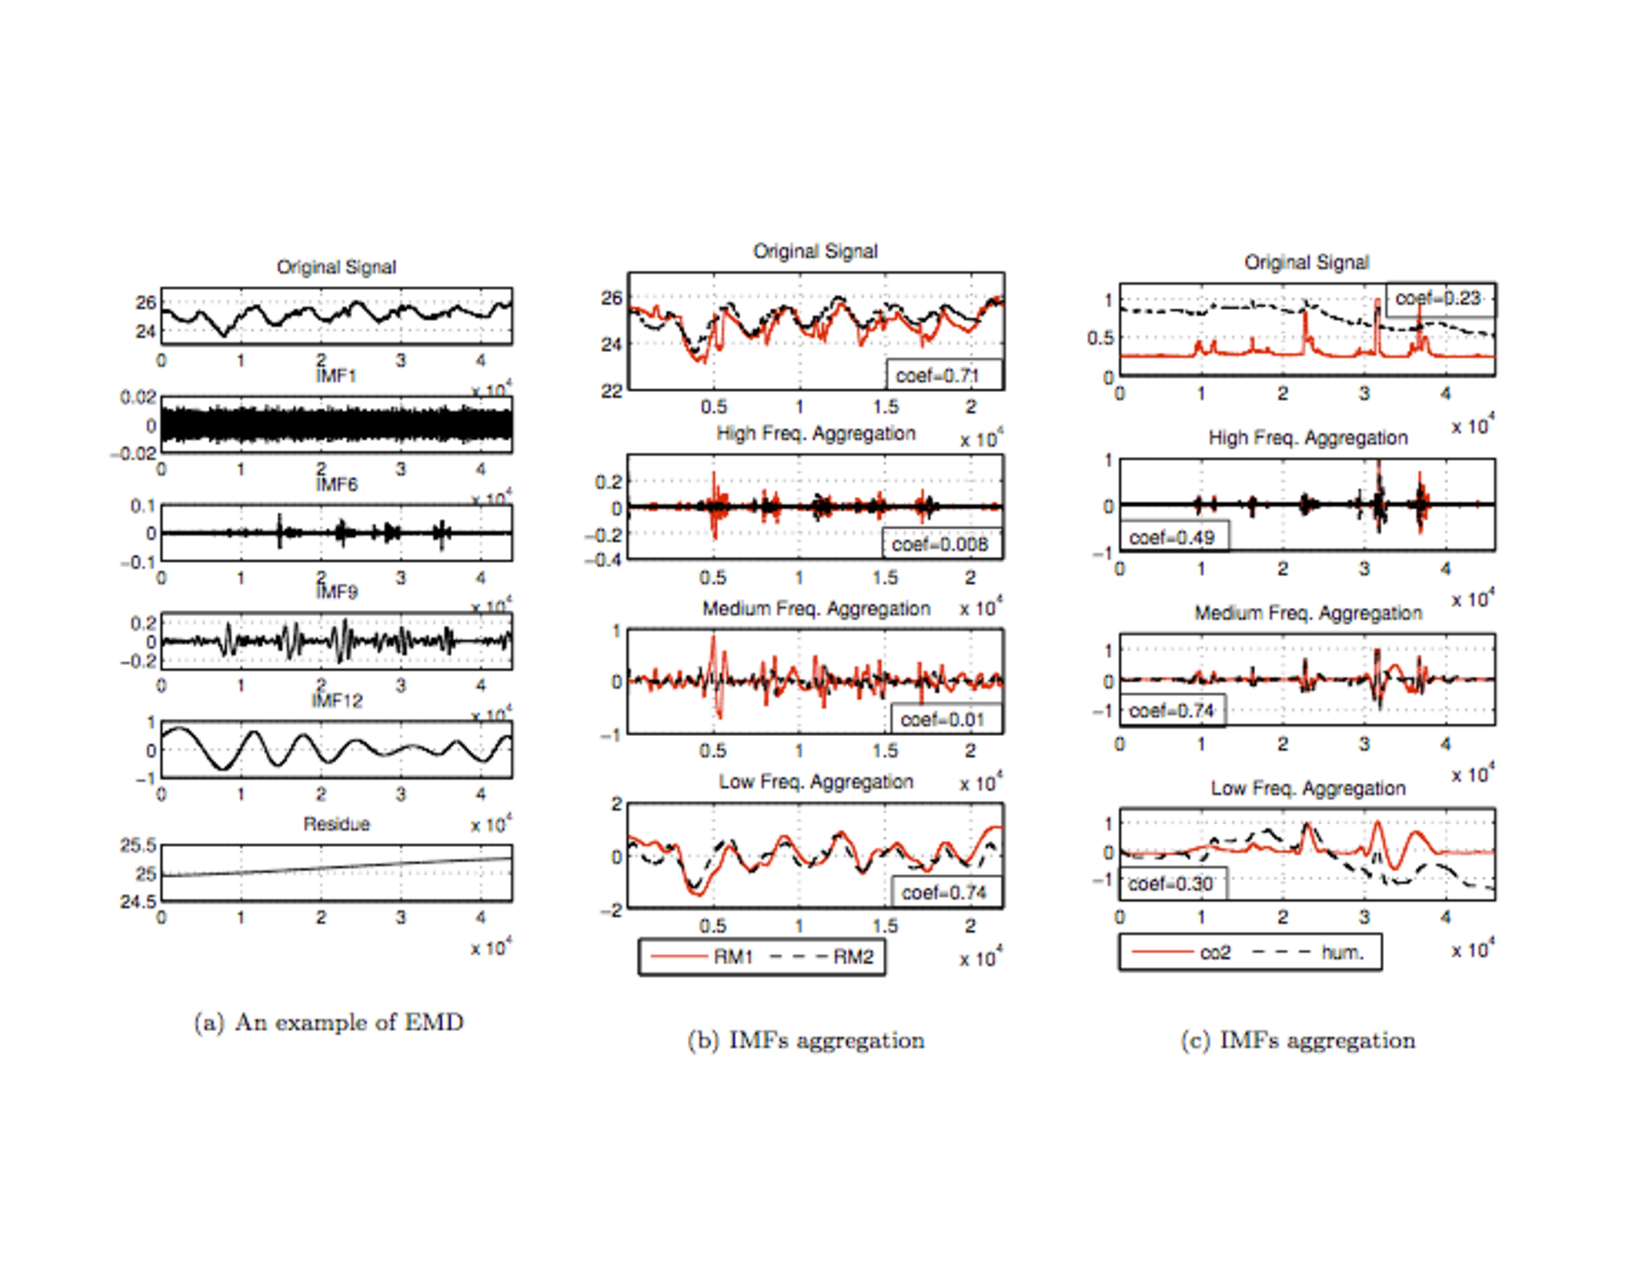
\includegraphics[width=0.95\textwidth]{figs/IMFReAggExample}
\caption{(a) EMD decomposes a signal and exposes intrinsic oscillatory components; (b) Aggregation of IMFs within a pre-defined frequency range makes seemingly similar signals from different locations more distinguishable; (c) IMF aggregation makes seemingly distinct signals of different sensors in the same room show high correlation.}
\end{figure*}

% We investigate the utility of empirical mode decomposition (EMD) to identify intrinsically
% correlated usage patterns among sensors in a large deployment.  We use data collected from almost $700$
% sensors in a 12-story building measuring power, pressure, temperature, and other physical
% phenomena.  We discover that doing a correlation analysis on the raw traces does not discriminate well enough
% to identify meaningful relationships between sensors.  We correlate the trace from a pump with the rest of
% the sensor traces and find that simple correlation filters only $50\%$ of the sensors as being correlated
% with the behavior of the pump. 
% In contrast, by running the correlation analysis on the constituent frequencies extracted by
% the EMD process, we filter out over $99\%$ of the sensors as being correlated -- with the highest correlation coming 
% from sensors that serve the same room as the pump.  We believe our approach can be used to 
% construct inter-device correlation models that can help understand and identify misbehaving or inefficient
% usage patterns.

% We present results for correlating usage patterns across a large number of sensors
% in a single deployment.  We analyze data from a 12-story office building at the University of Tokyo.  
% The deployment consists of almost 700 sensors monitoring a broad range of devices inside and outside 
% the building.  Our initial observations and results include the following:

% \begin{enumerate}
% \item Raw-trace correlation analysis is too strongly influenced by the common low-frequency trends in the data
% 	to identify meaningful relationships.
% \item Using a technique called empirical model decomposition (EMD)~\cite{huang:emd1998} removes this 
% 		 trend and helps identify truly correlated sensor traces.
% \item We can construct clusters of correlated sensors that are spatio-temporally correlated, \emph{without
% 		a priori knowledge of their placement}.
% \end{enumerate}



% Prior work~\cite{IOT} makes use of a technique called Empirical Mode Decomposition (EMD)~\cite{EMD} to statistically cluster correlated
% usage patterns.  Sensors close to each other show strong statistical correlations while sensors further apart show weaker correlations.  
% The main parameter in their approach, the correlation threshold, is explored to demonstrate how it relates to characteristic spatial patterns
%  in the sensor feeds.  However, they do not characterize the threshold as it relates to physical configuration.
% Fontugne et al.~\cite{SBS} expand the work by applying EMD to uncover functional device patterns.  They develop
% an unsupervised learning method to model normal usage patterns and apply an anomaly detection algorithm to alert when patterns
% have deviated from the norm.  The methodology used in their work divides raw signals into four separate frequency bands
% and shows the medium band to carry the most spatial information.

% In this section, we explore the threshold parameter in~\cite{IOT} more deeply, in order to move towards automatic spatial clustering, 
% to be used as a form of verification. We use EMD and the intrinsic mode function (IMF) re-aggregation methodology described in~\cite{SBS}, with some modifications, to statistically analyze the threshold parameter
% and its relationship to spatial separation in a building.  We explore the hypothesis that \emph{a statistical boundary, analogous to a physical one,
% exists and is empirically discoverable}.
% We conduct an empirical analysis on the data collected from 15 sensors in 5 rooms over a one-month period.  Our study makes the following contributions:

% \begin{itemize}
% \item We corroborate the results in~\cite{IOT}, verifying the spatial correlation pattern in a very different building.
% \item We characterize the correlation coefficient (corrcoeff) distribution of sensors in the same room and different rooms and validate our existence hypothesis for this preliminary sample.
% \item We demonstrate that the statistical boundary between sensors in various rooms converges to a similar value and this value generalizes across rooms in this study.
% \item We show the tradeoff between the true and false positive rate inherent to threshold selection. We also show that our method improves the classification accuracy from 80\% to 93.3\%.
% \end{itemize}

% Our results are promising yet preliminary.  We are able to find a statistical separation across a small number of rooms, quite well.
% Our study, however, does not explore the extent to which the physical separation affects the results.  Certainly for rooms that
% are far apart we observe a statistical distinction using our methodology.  However, we also find that in some cases, our approach
% does not work as well.  We discuss the approach and results in the rest of the paper, followed by a short discussion and future work.


We start our analysis by extending the methodology used for functional verification, based on empirical mode decomposition (EMD).  
In our analysis, we collect traces from several sensors and run EMD on them.  This produces a set of 
``intrinsic mode functions'' (IMF), which we separate by frequency range and re-aggregate them into distinct bands.
Then, we inspect the relationship between the sensors by computing the corrcoeff within a particular band, which 
gives us the spatial information we are interested in. 
Finally, we separate the result set into sub-sets, and closely examine their statistical characteristics. 
% Before describing our methodology in detail, we introduce some definitions and notation.



\subsection{Categorical Verification}
Categorical verification is the ability to cluster sensor traces by the type of sensor that it (i.e. its unit of measure) and the thing it is measuring.
Ideally we should be able to separate feeds that are measuring different physical attributes and/or are placed in different parts of the building.
For example, if there are sensors measuring temperature in a pipe and temperature in a room we should be able to separate them from one another as well
as separate them from sensor pressuring pressure in a valve.  We will show that this can be by examining their distribution and for 
small data sets with different sensor our approach works quite well, however we present some challenges in a large, more realistic deployment
data set and we discuss why it is so challenging to deal with.


% \subsection{Value Verification}
% Value verification used a physical model to verify that the value observed in the given context is producing values that agree with the model
% that is based on first-principles.  We do not explore this problem in this thesis and leave it for future work.


% \section{Building Datasets}

In this thesis, we run all of our experiments and analysis on data from the four buildings.  They serve as 
the main sites for experiemental data collection and/or sites from which we obtained data dumps from their building
management system.

% In addition, we expect the anomaly detector to identify discontinuities in these relationships that represent obvious electricity saving opportunities (e.g. a room HVAC left on during night while the room lights have been turned off).

% Due to privacy concern this dataset is not publicly available on the Internet but accessible upon request.


\subsection{Engineering Building 2 - Todai}\label{data:engbldg2}
%The data from building 1 is collected at the Engineering Building 2 of the Hongo campus. 
Engineering building 2, at the University of Tokyo (Todai), is a 12-story building completed in 2005.  It contains
classrooms, laboratories, offices and server rooms.  
The electricity consumption of the lighting and HVAC systems of 231 rooms is monitored by 135 sensors.
Rather than a centralized HVAC system, small, local HVAC systems are set up throughout the buidling.  
The HVAC systems are classified into two categories, EHP (Electrical Heat Pump) and GHP (Gas Heat Pump).
The GHPs are the only devices that serve numerous rooms and multiple floors.  The 5 GHPs in the dataset serve 154 rooms.
The EHP and lighting systems serve only pairs of rooms and which are directly controlled by the occupants.
In addition, the sensor metadata provides device-type and location information (room number), 
therefore, the electricity consumption of each pair of rooms is separately monitored.


\section{Related work}

%\begin{itemize}
% \item dashboard
% \item andrew's lightin control work
% \item Kamin's hvac control work
% \item BEMs
% \item sMAP stuff
%\item Buildsys 2010 work~\cite{hbci}
%\item distributed consistency management: COPS
%\item mobility: tracking things with RFID~\cite{rfid_gonz2006}
%\item mobility: tracking of people, wifi indoor localization
%\item entity-relationship graphs
%\item homeOS [microsoft]
%\item HP Cooltown~\cite{cooltown}
%\end{itemize}
Our work touches on several areas from smart home research to logistics.  In the building space, there has been
some interest in building various kinds of energy-related visual and control applications.
This work focuses on the object definition, tracking, and management component of the architecture proposed by 
Hsu et al.~\cite{hbci}.  Their work stratefied the set of challenges that one could potentially face if the application 
were deployed at scale.  Our
work, in constrast, bases its design rationale on a \emph{real deployment} that is taking place at scale in a building 
on our campus.  We focus on solving fundamental systems challenges in dealing with intermittent connectivity
and conflict resolution in tracking people and things over time.  We also focus on leveraging gestures to minimize
the cost of interaction for users, while maximizing the information we can attain about the state of the world.

% Tracking people/indoor localization
An important aspect of the Energy Lens is determining when people and things have moved.  This requires some form 
of indoor localization.  There's a large body of literature in the area of indoor localization with mobile phones ranging from 
using wifi~\cite{radar}, to sonar~\cite{cricket}, to ambient noise~\cite{abs}, and a combination of sensors on the 
phone~\cite{surroundsense, darwinphone}.  Dita~\cite{dita} uses acoustic localization of mobile phones and also uses the infrastructure 
to determine gestures in free-space that are classified into pre-defined control actions.  Each of these require relatively complex 
software and/or infrastrure.  
We take a radically different, simple approach.  We use cheap, easy to re/produce tags (QR codes), place them on things in the 
environment over incrementally and use the natural \emph{swiping gesture} that users make, when interacting with the Energy Lens 
application, to track when they have moved or when the objects around them have moved.  The working principal is to attain as much 
information from their gesture to determine when something/one has moved.  We discuss our heuristics in section~\ref{sec:swipes}.

% context-aware apps
ACE~\cite{ACE} uses various sensors on the phone to infer a user's context.  The context domain consists of a set of user activities
and semantic locations.  For example, if ACE can distinguish between {\tt Running, Driving, AtHome, or InOffice}.  ACE also infers 
the one from the others, so if the user is {\tt AtHome} then they are not {\tt InOffice}.  Energy Lens uses inference to determine
when a person or thing has moved.  Certain swipe combinations give us information about whether they moved and where they moved to or
whether an item moved and where it moved to.  The main difference is that we only infer context when a user is actively swiping, rather
than a continuous approach.  Pretching is a fundamental technique used in many domains.  However, the cost of a prefetch for mobile
application outways the benefits if the prefetched data is not useful.  Informed mobile pretching~\cite{IMP} uses cost-benefit analysis 
to determine when to prefetch content for the user.  In the Energy Lens context, we prefetch data based on their location swipes.
We also rely on pretching to anticipate loss of connectivity, not just to improve preformance.

% Tracking things
Logistic systems focus on the tracking of objects as the move through distribution sites to warehouses, stores, shelves,
and purchase.  Items are tracked through bar code or RFID readers.  However, the workload is very structured and well
defined.  The authors of~\cite{rfid_gonz2006} describe this structure and leverage it to minimize storage
requirements and optimize query-processing performance.  Energy Lens uses the QR codes as the tag and the phone as an active
reader.  As objects move, users scan those items to their new location.  However, objects may belong to one or
many people, they can be metered by multiple meters a day, and their history in the system
is on-going.  In contrast, a typical logistics workload has a start (distribution site) and end point (leaving the store
after a sale).  In our workload, relationship semantics are important; we need to know whether the meter is \emph{bound-to}
rather than simple \emph{attached-to} an item.  We discuss the difference later in the paper.
% In addition to traditional logistics-style queries -- \emph{What is the average time that it took coffee-makers to move from the 
% warehouse to the shelf and finally to the checkout counter in January of 2004?} -- energy-analytics requires queries to group
% partial traces from meter data by tracking what meters the item attached to over the specified time-frame.
% The Energy Lens system collects and manages this kind of information to enable such queries.
Furthermore, we take advatange of natural gestures the user makes with the phone while scanning QR codes to extract
information about the current location of the user or things.

% Tagging items, virtual services
The key idea in the HP Cooltown~\cite{bridgingphysical,cooltown} work is to web-enable `things' in the world, grouped-by
`place', and accessed by `people' via a standardized acquisition protocol (HTTP) and format (HTML, XML).  
Cooltown creates a web presence for things in the world either directly (embedded web server) or indirectly 
(URL-lookup tag) as a web page page that display the services it provides.  Many of the core concepts in Cooltown 
also show up in Energy Lens.  The main overlap is the use of tags in the world that contain a reference to a virtual 
resource, accessible via HTTP through
a network connection.  Cooltown, however, explicitly chooses not maintain a centralized relationship
graph, it leverages the decentralized, linking structure of the web to group associated web pages together.
Furthermore, things are assumed to not move.  People are the main mobile entities.  The kind of applications
we wish to support must track where things are and their specific inter-relationships.  We imposed a richer set of 
semantics on our, centrally maintained, relationship graph and use it to provide detailed energy information.


\section{Summary}

% StreamFS consists of over 20,000 lines of code and was implemented in mostly Java.  It was deployed across multiple
% buildings and several applications were built on top of it over a 2 years period.

In this chapter we gave an overview of the main components in StreamFS.  Each of the components addresses the concerns stated in 
section~\ref{sec:shortcomings}.  The filesystem name server expose a uniform namespace for access sensors and actuators in 
deployed throughout the building.  The timeseries database serve to store data streaming physical information and 
is optimized for the scan-style queries posed by applications.  These address points \ref{nw} and \ref{ts}.
We also include a pub-sub system which serves multiple purposes.  It provides real-time data forwarding for external
applications and forwards data internally to processing units that are specified or linked by the user.
This addresses points \ref{rt}.  Finally, we introduce processing elements, both internal and external to address
point \ref{proc}.  We also introduce an entity-relationship graph to deal with indirect relationships that are
expressed in the construction of names in the system.

In the next chapter we talk more about processing and discuss the details in the scheduler that help enable applications
that have certain delivery requirement.

\section{Summary}

% StreamFS consists of over 20,000 lines of code and was implemented in mostly Java.  It was deployed across multiple
% buildings and several applications were built on top of it over a 2 years period.

In this chapter we gave an overview of the main components in StreamFS.  Each of the components addresses the concerns stated in 
section~\ref{sec:shortcomings}.  The filesystem name server expose a uniform namespace for access sensors and actuators in 
deployed throughout the building.  The timeseries database serve to store data streaming physical information and 
is optimized for the scan-style queries posed by applications.  These address points \ref{nw} and \ref{ts}.
We also include a pub-sub system which serves multiple purposes.  It provides real-time data forwarding for external
applications and forwards data internally to processing units that are specified or linked by the user.
This addresses points \ref{rt}.  Finally, we introduce processing elements, both internal and external to address
point \ref{proc}.  We also introduce an entity-relationship graph to deal with indirect relationships that are
expressed in the construction of names in the system.

In the next chapter we talk more about processing and discuss the details in the scheduler that help enable applications
that have certain delivery requirement.


